\documentclass[Bachelor, USenglish]{scrbook}
%------------------------------------------------------------------------------
% This file contains a skeleton thesis for
% a Physics or Astronomy Institute in the University of Bonn.

% Specify the thesis type as an option: PhD, Master, Diplom, Bachelor.
% Specify the thesis stage as an option: Draft (default), Submit, Final, PILibrary.

% Specify the language(s) in the class and then use babel.
% If you need more than one language, give the default language last,
% e.g. ngerman, UKenglish for a thesis in British (UK) English where you want
% to be able to set the language to German for some part of it.

%------------------------------------------------------------------------------
% Pass TeX Live version to the package.

% twoside=true is suitable for printing, while twoside=false is probably better for PDF version.
% Pass option refsection=none if you want the bibliography at the end of the thesis.
\usepackage[twoside=false, astrobib, refsection=none, todonotes=true]{ubonn-thesis}

%------------------------------------------------------------------------------
% Adjustments to standard biblatex style.
% Change option to backref=false when your thesis is ready to turn off back-referencing.
% Pass the option showurl=false to shorten your bibliography by not including url fields.
% Astronomy theses usually set block=none. block=ragged is the default.
\usepackage[backref=true, block=none]{ubonn-biblatex}

%------------------------------------------------------------------------------
% Glossary package
% \usepackage[acronym,toc,nosuper]{glossaries}
% TikZ packages and libraries
% \usepackage{tikz}
% \usepackage{tikz-3dplot}
% \usepackage{pgfplots}
% \usetikzlibrary{positioning,shapes,arrows}
% \usetikzlibrary{decorations.pathmorphing}
% \usetikzlibrary{decorations.markings}
\usepackage{thesis_defs}

%------------------------------------------------------------------------------
% Instead of colouring  links, cites, table of contents etc.
% put them in a coloured box for the screen version.
% This is probably a good idea when you print your thesis.
% \hypersetup{colorlinks=false,
%   linkbordercolor=blue,citebordercolor=magenta,urlbordercolor=darkgreen
% }

%------------------------------------------------------------------------------
% When writing your thesis it is often helpful to have the date and
% time in the output file. Comment this out for the final version.
\ifoot[\today{} \thistime]{\today{} \thistime}

% In order to check if your labels are referenced try the refcheck package
% \usepackage{refcheck}

%------------------------------------------------------------------------------

% Specify the bibliography files 
\addbibresource{bib/thesis_refs.bib}

%------------------------------------------------------------------------------
% The following definitions are used to produce the title pages
% needed at various stages
\newcommand{\thesistitle}{INSERT CREATIVE NAME HERE}
\newcommand*{\thesisauthor}{Author's name}
\newcommand*{\thesistown}{Place of birth}
\renewcommand*{\InstituteName}{\AIFA}
\renewcommand*{\inInstitute}{\inAIFA}
\renewcommand*{\InstituteAddress}{\PIaddress}
% Adjust \thesisreferee...text depending on male/female referee
\newcommand*{\thesisrefereeonetext}{1.\ Gutachter}
\newcommand*{\thesisrefereeone}{Prof.\ Dr.\ John Smith}
\newcommand*{\thesisrefereetwotext}{2.\ Gutachterin}
\newcommand*{\thesisrefereetwo}{Prof.\ Dr.\ Anne Jones}
% Date when thesis was submitted (Master/Diplom)
% Year or Month, Year when thesis was submitted (PhD)
\newcommand*{\thesissubmit}{XX.YY.2024}
% \newcommand*{\thesissubmit}{Month 2024}
% Date of thesis examination (PhD)
\newcommand*{\thesispromotion}{XX.YY.2024}
% Month and year of the final printed version of the thesis
\newcommand*{\thesismonth}{MMM}
\newcommand*{\thesisyear}{2024}
\newcommand*{\thesisnumber}{BONN-IR-2024-XXX}
% Dedication
% \newcommand*{\thesisdedication}{}

%------------------------------------------------------------------------------
% The abstract is only needed for the printed version and should be in
% English regardless of the language of the thesis
\newcommand{\thesisabstract}{%
  \begin{otherlanguage}{UKenglish}
    This is your thesis abstract. It may be in a language that is
    different from the rest of your thesis.
  \end{otherlanguage}
}

%------------------------------------------------------------------------------
% \includeonly can be used to select which chapters you want to process
% A simple \include command just inserts a \clearpage before and after the file
% Note that \includeonly can be quite picky! Do not forget to put a
% comma after the filename, otherwise it will simply be ignored!
\includeonly{%
  thesis_intro,
  thesis_theoretical_background,
  thesis_data_reduction,
  thesis_analysis,
  thesis_conclusion,
  thesis_appendix,
  thesis_acknowledge,
  thesis_appendix_a
}

%------------------------------------------------------------------------------
% Give a list of directories where figures can be found. Do not leave
% any spaces in the list and end the directory name with a /
\graphicspath{%
  {figs/}%
  {figs/cover/}%
}

%------------------------------------------------------------------------------

% Draft version - add the word DRAFT on the cover pages
% Also add the date and time of compilation and turn on line numbers (if option is set).
\ifthenelse{\equal{\ThesisVersion}{Draft}}{%
  \usepackage{background}
  \backgroundsetup{contents=DRAFT, color=blue!30}
  \ifoot[\today{} \thistime]{\today{} \thistime}
  \ifthenelse{\boolean{ThesisLineno}}{\linenumbers}{}
 }

%------------------------------------------------------------------------------
\begin{document}

% Make cover and title pages
\makethesistitle

\pagestyle{scrplain}

%------------------------------------------------------------------------------
% You can add your acknowledgements here - don't forget to also add
% them to \includeonly above
%------------------------------------------------------------------------------
\chapter*{Acknowledgements}
\label{sec:ack}
%------------------------------------------------------------------------------

I would like to thank ...

You should probably use \texttt{\textbackslash chapter*} for
acknowledgements at the beginning of a thesis and
\texttt{\textbackslash chapter} for the end.

%%% Local Variables: 
%%% mode: latex
%%% TeX-master: "../mythesis"
%%% End: 


\tableofcontents

\mainmatter
\pagestyle{scrheadings}

% Turn off DRAFT for the following pages
\ifthenelse{\equal{\ThesisVersion}{Draft}}{%
  \backgroundsetup{contents={}}
}{}

%------------------------------------------------------------------------------

% !TEX root = mythesis.tex

%==============================================================================
\chapter{Introduction}
\label{sec:intro}
%==============================================================================
Unlike the larger and more massive galaxy clusters, galaxy groups are smaller systems with typical masses around \(3 \times 10^{13} M_{\odot}\) (\cite{Schneider_2006}). Despite their relative modesty, the study of galaxy groups is fundamental to our understanding of the Universe's large-scale structure (LSS), as they likely contain a significant fraction of the total baryonic mass in the Universe (\cite{Peebles1998}). Galaxy clusters and galaxy groups are characterized by a hot, ionized gas known as the intracluster medium (ICM) or the intragroup medium (IGM), which fills the space between the galaxies. This gas emits copius amounts of X-rays making X-ray observations an essential tool for identifying and studying these structures (\cite{KravtsovBorgani2012}).

The galaxy group NGC1550, first linked to the extended X-ray source RX J0419+0225 through the ROSAT All-Sky Survey (\cite{Bohringer_2000}), has been the subject of extensive X-ray analysis. Observations have been conducted using various instruments, including ASCA (\cite{Kawaharada_2003}), XMM-Newton (\cite{Kawaharada_2009}), Chandra (\cite{Sun_2003}), and Suzaku (\cite{Sato_2010}). In this thesis, data from the \textit{extended ROentgen Survey with an Imaging Telescope Array} (eROSITA) shall be utilized characterize the X-ray surface brightness profile of NGC1550 and compare the results with previous studies.

Following a brief overview of the theoretical background in Chapter \ref{sec:theoretical_background}, Chapter \ref{sec:data_reduction} will focus on reducing and correcting the data for various effects. Chapter \ref{sec:data_analysis} will analyze the surface brightness profile of NGC1550, including detailed assessments and a beta model fitting of the full azimuthal profile. Additionally, the analysis will compare the north, south, east, and west sectors against each other and against the full azimuthal profile. Finally, Chapter \ref{sec:conclusion} will present the thesis conclusions, and Chapter \ref{sec:outlook} will summarize all results, offer suggestions for of the analysis and for future works.

%------------------------------------------------------------------------------

% !TEX root = mythesis.tex

%==============================================================================
\chapter{Theoretical Background}
\label{sec:theoretical_background}
%==============================================================================
\section{Clusters and Groups of Galaxies}\label{sec:clusters}
Throughout the Universe, galaxies are not distributed homogeneously but are instead aggregated into large cosmic structures known as galaxy groups or galaxy clusters, which are the largest virialized structures in the Universe. Galaxy clusters typically have masses exceeding \(M \gtrsim 3 \times 10^{14} M_{\odot}\), whereas galaxy groups have masses around \(M \sim 3 \times 10^{13} M_{\odot}\) (\cite{Schneider_2006}). Advancements in X-ray astronomy have demonstrated that these structures are significant sources of X-ray radiation (\cite{Cavaliere_1971}). This emission is well understood to originate from a hot intergalactic gas known as the intracluster medium (ICM)\footnote{The intercluster medium is also called the intragroup medium (IGM) in the case of galaxy groups. In the context of this thesis, the terms ICM and IGM will be used interchangeably, as a distinction between them is not necessary.}, which is characterized by temperatures in the range of \SIrange{e7}{e8}{\kelvin} and constitutes the primary baryonic component of galaxy clusters and groups (\cite{Schneider_2006}).
%
\subsection{The Intracluster Medium}
Within the deep gravitational wells of galaxy clusters and groups, the temperature becomes sufficiently high to fully ionize lighter elements and partially ionize heavier elements, resulting in the formation of a plasma. This hot, diffuse, and optically thin plasma, known as the intracluster medium (ICM), emits a significant amount of X-ray radiation. X-ray observations of the ICM have enabled a wide variety of cosmological studies including advances in understanding the large-scale structure formation in the Universe (\cite{KravtsovBorgani2012}).
%
\subsection{Emission Processes within the ICM}\label{subsec:emission}
A key principle of electrodynamics is that accelerated charges radiate energy. This radiation is referred to as bremsstrahlung or \enquote{free-free} when a unbound charged particle, typically an electron, is accelerated by the electric field of other charges, usually ions. In the ICM, this process predominates at temperatures above \(k_B T_\text{e} \gtrsim \SI{2}{\kilo\electronvolt}\), where the total emissivity \(\epsilon_{\text{ff}}\) at solar metallicity scales approximately as \(\epsilon_{\text{ff}} \propto T_\text{e}^{0.5} n_\text{e}^2\), 
with \(n_\text{e}\) and \(T_\text{e}\) as the electron number density and temperature, respectively. At lower temperatures (\(k_B T \lesssim \SI{2}{\kilo\electronvolt}\)), line emission becomes significant, with the emissivity being roughly described by \(\epsilon \propto T_\text{e}^{-0.6} n_\text{e}^2\).
Thus, for the low energy band \SIrange{0.1}{2.4}{\kilo\electronvolt}, one has a weak temperature dependence, i.e. \(\epsilon \propto n_\text{e}^2.\) (\cite{Reiprich2019}).
%
\subsection{The \(\beta\)-model of the ICM}\label{sec:beta_model}
In the mid-1970s, \citep{Cavaliere_1976} laid the groundwork for the current understanding of the ICM. The X-ray morphology of clusters and groups is typically described by the beta model. This model assumes gas and galaxies share the same gravitational potential. Given a constant temperature \(T\) and velocity dispersion \(\sigma_r\), the radial distributions of the gas \(n_{\text{gas}}\) and galaxies \(\rho_{\text{gal}}\) obey
\begin{align*}
    \frac{n_\text{gas}(r)}{n_{\text{gas}}(0)} = \left[\frac{\rho_{\text{gal}}(r)}{\rho_{\text{gal}(0)}}\right]^{\beta}; \quad \beta = \frac{\mu m_\text{p} \sigma_r^2}{k_\text{B}T}
\end{align*}
where \(\mu\) is the mean molecular mass, \(m_p\) is the proton mass and \(k_B\) is the Boltzmann constant. Using the King approximation \({\textstyle \rho_{\text{gal}}(r) = \rho_{\text{gal}}(0)[1 + (r/r_c)^2]^{-3/2}}\) (\cite{King1962}), where \(r_c\) is the core radius and \(\epsilon \propto n_e^2\), the X-ray surface brightness \(S_X\), obtained by integrating over the emissivity, follows the profile 
\begin{align*}
    S_X(r) = S_X(0)\left[1 + \left(\frac{r}{r_c}\right)^2\right]^{-3\beta + 1/2}.
\end{align*}
The beta model is widely used to describe cluster and group emissions, despite the assumptions listed above often being unmet. Excess core emission, for example, is typically addressed by adding a second beta model component: \(S_X^{\text{tot}} = S_{X,1} + S_{X,2}\) (\cite{Reiprich2019}).
%
\subsection{The galaxy group NGC1550}\label{sec:ngc1550}
The galaxy group NGC1550 is located at a right ascension of \(\SI{64.9066}{\degree}\) and a declination of \(\SI{2.4151}{\degree}\), with a redshift of \(z = 0.0123\) (\cite{Reiprich_2002}). Although the lenticular galaxy NGC 1550 has long been observable in the optical, it was first associated with the extended X-ray source RX J0419+0225 through the ROSAT All-Sky Survey (\cite{Bohringer_2000}). The presence of this extensive X-ray halo, along with its considerable mass (\(\sim 2 \times 10^{13} M_{\odot}\)), led to its classification as a galaxy group (\cite{Kawaharada_2003}).

Recent studies indicate that NGC1550 does not meet the formal criteria for a fossil group (\cite{Sun_2003}; cf. \cite{Jones2003} for the criteria), but it shares several features with such groups. One notable characteristic is its high X-ray bolometric luminosity (\(\gtrsim \SI{4.8e41}{\erg}\)), which predominantly originates from a central, dominant, early-type galaxy. Fossil groups are thought to be formed when member galaxies in a regular galaxy group merge into a central dominant galaxy, and evidence for this process has been found in the metal distribution of NGC1550 (\cite{Kawaharada_2009, Sato_2010}). Additionally, a recent study has identified signs of AGN (active galactic nucleus) feedback and sloshing, suggesting a minor merger occurred around 33 million years ago (\cite{Kolokythas_2020}). While the group appears to be relaxed overall, a slight east-west elongation in the central region has been noted by multiple authors (\cite{Kolokythas_2020, Sun_2003}).
%
\section{eROSITA}
The \textit{extended ROentgen Survey with an Imaging Telescope Array} (eROSITA) is a highly sensitive, wide-field X-ray telescope designed to capture deep images across large areas of the sky. Mounted on the Spektrum-Roentgen-Gamma (SRG) observatory in a halo orbit around the second Lagrange Point (L2), eROSITA operates within the 0.2 to 10.0 keV energy range. It is the first instrument to perform an all-sky imaging survey in the hard X-ray band (2.0 to 10.0 keV). In the soft X-ray band (0.5 to 2.0 keV), eROSITA boasts a sensitivity greater than that of its predecessor, the ROSAT All-Sky Survey. eROSITA features seven identical mirror modules, known as Telescope Modules (TMs), with 54 mirror shells in Wolter-I geometry and a 1.6-meter focal length. Five TMs (TM1, TM2, TM3, TM4 and TM6) have aluminum on-chip optical light filters and are collectively referred to as TM8. The remaining two TMs (TM5, TM7), designed for low-energy spectroscopy, lack these filters and are referred to as TM9. Collectively, TM8 and TM9 are referred to as TM0. (\cite{Predehl2021}). In this thesis, data from the first all-sky survey (eRASS:1) will be utilized. The data is provided in the form of event lists, which essentially detail the spatial position of X-ray photon arrivals on the detector, their time of arrival, and their energy. The event lists are made available in \(\SI{3.6}{\degree}\times\SI{3.6}{\degree}\) regions known as skytiles.
\section{Sky background and contamination sources}\label{sec:background}
For a thorough analysis of X-ray photons, it is essential to carefully consider both external background and internal instrumental contamination effects. The following section will provide a brief overview of the most important factors relevant to this analysis.
\paragraph*{Cosmic X-ray Background (CXB):} The cosmic X-ray background (CXB) comprises multiple sources, including diffuse, unabsorbed thermal emissions from the Local Hot Bubble, a plasma cavity surrounding the Sun, and absorbed thermal emissions from the Galactic halo (\cite{galeazzi2006xmm}). Additionally, it includes discrete extragalactic sources, predominantly unresolved AGNs  (\cite{brandt2005deep}). The diffuse component is more prominent in the lower energy band \(\sim\SI{1}{\kilo\electronvolt}\), while the extragalactic sources dominate at higher energies. In this analysis, background emission from the nearby Orion-Eridanus superbubble, which spans roughly \SI{40}{\degree} on the sky, shall also be present, as it emits in the soft X-ray regime (\cite{Krause_2014}). Figure \ref{fig:orion_superbubble}, taken from \citep{Krause_2014}, shows an X-ray map of the Orion-Eridanus superbubble in the \SIrange{0.5}{2.0}{\kilo\electronvolt} band, illustrating its overlap with the emission from the galaxy group NGC1550.
\begin{figure}[htbp]
    \centering
    \includegraphics[width=0.7\textwidth]{data_reduction/rosat_orion_supper_bubble.png}
    \caption{X-ray map in galactic coordinates of the Orion-Eridanus superbubble in the \SIrange{0.5}{2.0}{\kilo\electronvolt} band from the ROSAT all-sky survey. The colorbar units are \(10^{-6}\,\text{cts}\cdot\text{arcmin}^{-2}\text{s}^{-1}\) and the contour levels are 220, 300, 380,
    460, 540, 620, 700. The image was taken from \citep{Krause_2014}. The green arrow and label were added to highlight the position of NGC1550.}
    \label{fig:orion_superbubble}
\end{figure}
\paragraph*{Non-X-ray Background (NXB):} The non-X-ray background consists of two main components: highly variable soft protons flares (SPF) from the solar corona and Earth's magnetosphere, which can be focused onto detectors, and energetic Galactic Cosmic Ray (GCR) primaries, which interact with the detector to produce secondary particles. The secondary particles can deposit charge in the detector, making it challenging to distinguish them from true X-ray events. This is generally referred to as the particle-induced background (PIB) (\cite{Bulbul_2020}). 
\paragraph*{eROSITA light leak:} Shortly after the launch of eROSITA, it was observed that CCDs lacking an on-chip filter (TM9) recorded a notably higher number of events. This was attributed to optical and ultraviolet light from the Sun entering the CCD through an unidentified gap in the detector shielding, and was subsequently termed \enquote{light-leak} (\cite{Predehl2021}).
\paragraph*{\(N_\text{H}\) absorption:} 
As X-rays travel to the detector, they undergo photoelectric absorption in the interstellar and intergalactic medium. The cross-section \(\sigma \propto E^{-3}\) is inversely proportional to energy, causing a bias toward harder X-rays, as they interact less. Additionally, the cross-section is proportional to the atomic number, \(\sigma \propto Z^5\), making metal abundance crucial for energies \(\gtrsim \SI{0.2}{\kilo\electronvolt}\) (\cite{Willingale2013}).



%------------------------------------------------------------------------------

% !TEX root = mythesis.tex

%==============================================================================
\chapter{Data Reduction}
\label{sec:data_reduction}
%==============================================================================
In the following section, the underlying data shall be reduced and corrected for the various effects and sources of contamination explained in Section \ref{sec:background}. Data from eRASS:1\footnote{\url{https://erosita.mpe.mpg.de/dr1/AllSkySurveyData_dr1/} (Last accessed: 05.08.2024)} and all TMs (1-7) is used, which were processed with the eROSITA pipeline processing version c010. The galaxy group NGC1550 is located in skytile 065087. Additionally, the surrounding skytiles 062084, 062087, 062090, 065084, 065090, 068084, 068087, and 068090 are used to cover regions up to \(\sim 3R_{200}\) (cf. value below). Data reduction is performed with the software HEASoft version\footnote{\url{https://heasarc.gsfc.nasa.gov/docs/software/heasoft/} (Last accessed: 04.08.2024)} 6.29 and the extended Science Analysis Software System\footnote{\url{https://erosita.mpe.mpg.de/dr1/eSASS4DR1/} (Last accessed: 04.08.2024)} (eSASS 4DR1). 

Values for \(R_{200}\) and \(R_{500}\) were taken from \cite{Reiprich_2002} and converted to \(R_{200} = 58.58'\) and \(R_{500} = 37.15'\) based on the cosmology used in this paper. The cosmology assumes \(\Omega_m = 0.3, \Omega_\Lambda = 0.7\) and \(h = 0.7\), with \(1'' = 0.252\,\text{kpc}\) at the redshift \(z=0.0123\) of the galaxy group. 
%The Matplotlib (\cite{Hunter:2007}) and Astropy (\cite{The_Astropy_Collaboration_2022}) Python packages were used to visualize the images.
\section{Raw photon images}\label{sec:raw_photon}
%
\begin{figure}[htbp]
    \centering
    \begin{subfigure}{0.325\textwidth}
        \centering
        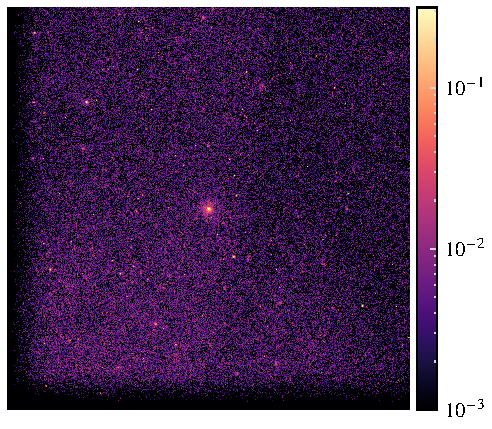
\includegraphics[width=\textwidth,height=\textwidth,keepaspectratio]{data_reduction/combined_tiles_0_raw_0.2-2.3keV.pdf}
        \caption{\SIrange{0.2}{2.3}{\kilo\electronvolt}}
        \label{fig:low_energy}
    \end{subfigure}
    \hfill
    \begin{subfigure}{0.325\textwidth}
        \centering
        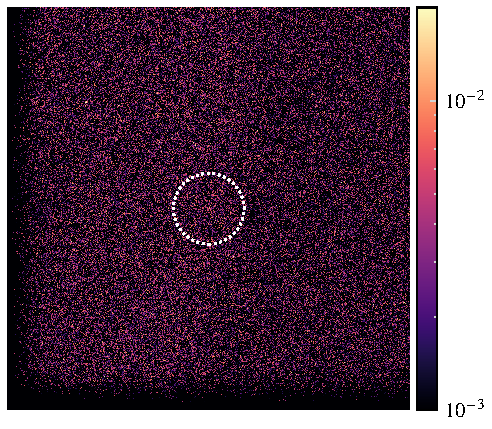
\includegraphics[width=\textwidth,height=\textwidth,keepaspectratio]{data_reduction/combined_tiles_0_raw_2.3-6.0keV.pdf}
        \caption{\SIrange{2.3}{6.0}{\kilo\electronvolt}}
        \label{fig:mid_energy}
    \end{subfigure}
    \hfill
    \begin{subfigure}{0.325\textwidth}
        \centering
        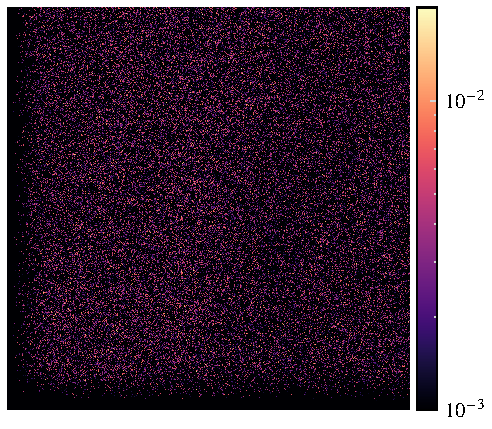
\includegraphics[width=\textwidth,height=\textwidth,keepaspectratio]{data_reduction/combined_tiles_0_raw_6.0-9.0keV.pdf}
        \caption{\SIrange{6.0}{9.0}{\kilo\electronvolt}}
        \label{fig:high_energy}
    \end{subfigure}
    \caption[Raw photon images from TM0 of all combined skytiles centered around NGC1550 displayed at different energy bands.]{Raw photon images from TM0 of all combined skytiles centered around NGC1550, displayed in the energy bands \SIrange{0.2}{2.3}{\kilo\electronvolt} (a), \SIrange{2.3}{6.0}{\kilo\electronvolt} (b), and \SIrange{6.0}{9.0}{\kilo\electronvolt} (c), with Gaussian smoothing of 4 pixels. The colorbar represents (smoothed) photon counts. For visualization purposes, different cuts were use for the middle and right image and \(R_{200}\) is shown (white dashed circle). The majority of the group emission is visible in the lower energy band (\SIrange{0.2}{2.3}{\kilo\electronvolt}).}
    \label{fig:raw_photon_images}
\end{figure}
%
Prior to the data reduction process, raw photon images for all combined skytiles and TMs are presented across the following energy bands: \SIrange{0.2}{2.3}{\kilo\electronvolt}, \SIrange{2.3}{6.0}{\kilo\electronvolt}, and \SIrange{6.0}{9.0}{\kilo\electronvolt}. The skytiles were combined using the \textit{eSASS} task \texttt{evtool} with no additional parameters applied to show all inherent deficiencies. The raw photon images are presented in Figure \ref{fig:raw_photon_images}. It is evident that the counts are noticeably lower in the right half of each image. This issue will be addressed in detail through the absorption and exposure correction in Section \ref{sec:exposure}. As can been observed, the group emission is mainly concentrated in the lower energy band, making the low energy band the focus for detecting emission structures. In this analysis, the \SIrange{0.2}{2.3}{\kilo\electronvolt} energy band is used. However, due to the light-leak in TM9 the energy range is restricted to \SIrange{0.8}{2.3}{\kilo\electronvolt}, while it remains \SIrange{0.2}{2.3}{\kilo\electronvolt} for TM8. Henceforth, this TM-dependent energy band will be referred to as the \enquote{soft-band} and the \SIrange{6.7}{9.0}{\kilo\electronvolt} energy range will be designated the \enquote{hard-band}. 
%
\section{Image filtering}
Each skytile is cleaned individually using \texttt{evtool} with \texttt{pattern=15} to select all event patterns (single, double, triple and quadruple) and \texttt{flag=0xe00fff30} to remove bad pixels and CCD corners. Subsequently, soft proton flares are identified and mitigated through the following process: the \texttt{flaregti} task is employed to generate light curves with \SI{20}{\second} time bins in the energy range of \SIrange{5}{10}{\kilo\electronvolt}. A \(3\sigma\) threshold is then determined; time intervals where count rates exceed this threshold are likely due to soft proton flares. Subsequently, the task \texttt{flaregti} is then rerun using the aforementioned threshold to establish good-time-intervals (GTIs) excluding these flare periods, which are applied using \texttt{evtool} with the \texttt{gti="FLAREGTI"} parameter. All SPF-filtered and cleaned skytiles are combined into a single TM0 photon image using \texttt{evtool}. From this point onwards, these combined images shall be referred to as \enquote{filtered}.
%
\section{Exposure map and image creation}\label{sec:exposure_map}
The \texttt{evtool} task, in conjunction with the \texttt{telid} parameter, is used to split the TM0 filtered photon images into individual filtered images for each TM. These images are then resized to the soft-band and the hard-band using \texttt{evtool} with the parameters \texttt{emin} and \texttt{emax}. Both vignetted and flat (non-vignetted) exposure maps are generated for each TM in the soft-band using the \texttt{expmap} task with the \texttt{withvignetting} parameter. These maps are utilized for subsequent PIB and exposure corrections. Moreover, the \texttt{withdetmaps} parameter is specified to crop the images at the edge of the field of view for each TM. By keeping \texttt{withmergedmaps} at its default value of \texttt{YES}, merged all-telescope exposure maps are created. This means the exposure maps consider the 7 TMs as one TM with on-chip TM, assuming the combined effective area of the 7 on-chip TMs. The vignetted and flat exposure maps are available in Appendix \ref{sec:appendix_a_exposure_map}.
\section{PIB Correction}\label{sec:pib_correction}
It is necessary to subtract the particle-induced background (PIB) from the combined filtered photon image. The following  approach is based on extensive studies of the eROSITA filter wheel closed (FWC) data conducted by Dr. F. Pacaud, as utilized for example in \citet{Reiprich2021}. The PIB is modeled for each TM using FWC data. Given the minimal spatial variation of the PIB, this modelling employs the flat exposure map created in Section \ref{sec:exposure_map}. Furthermore, due to the negligible spectral variation, the counts \(H_\text{obs}\) in the hard band, where PIB counts dominate, are used to estimate the PIB contribution in the soft-band by multiplication with the ratio \(R\) of the number of FWC counts in the soft band \(S_{\text{FWC}}\) to the hard band \(H_\text{FWC}\). The PIB-map for each TM is then generated by applying this factor to the flat exposure map, normalized to 1 by dividing by the sum of all pixel values (norm. flat exposure map). Therefore, the PIB map of a given TM is given by
\begin{align*}
    \text{PIB map}_\text{TM} = H_\text{obs}R\cdot\bigl(\text{norm. flat exposure map}\bigr).
\end{align*}
Soft-band, PIB-corrected image are obtained by subtracting the PIB map of each TM from the respective soft-band, filtered photon image. The complete image for TM0 is obtained by co-adding all PIB-corrected images. To better visualize the PIB-correction, individual background maps are also co-added to form a complete PIB map, which can be found in Appendix \ref{sec:appendix_a_pib_map}. Additionally, Appendix \ref{tab:values_of_R_and_H} contains the obtained \(H_\text{obs}\) and \(R\) values.
%
\section{Absorption Correction}
As previously outlined in Section \ref{sec:background}, X-ray absorption by the ISM must be taken into account. To correct for this absorption, the methodology outlined in \citet{Reiprich2021} is followed. Furthermore, scripts for the absorption correction were provided by Angie Veronica (as utilized in \cite{veronica2020}). At energies \(\gtrsim \SI{0.2}{\kilo\electronvolt}\), as is relevant for this analysis, the absorption of X-rays by metals play a significant role (cf. \ref{sec:background}). 
Assuming solar metallicity, the hydrogen column density \({\textstyle (N_\text{H})}\) can be used to trace the absorbing material. A cutout of the HI4PI all-sky survey (\cite{HI4PI2016}) is reprojected onto the field of view of the combined tile image to create a neutral atomic hydrogen map (\({\textstyle N_{\text{HI}}}\)-map). Additionally, as outlined in \citet{Willingale2013}, a molecular hydrogen map (\({\textstyle N_{\text{H}_2}}\)-map) is constructed by dividing the full sky image into \(52 \times 52\) pixel cells, querying \({\textstyle N_{\text{H}_2}}\) values from the Swift homepage\footnote{\url{https://www.swift.ac.uk/analysis/nhtot/index.php} (Last accessed: 25.07.2024)}, and distributing these values across each cell. The total hydrogen column density map,constructed by \({\textstyle N_{\text{Htot}} = N_{\text{H}} + 2N_{\text{H}_2}}\), is shown in Figure \ref{fig:NH_map}, with \({\textstyle N_{\text{H}}}\) ranging from \({\textstyle N_\text{Htot, min} = \SI{2.91e+20}{{\centi\meter}^{-2}}}\) to \({\textstyle N_\text{Htot, max} = \SI{1.61e+21}{{\centi\meter}^{-2}}}\).

Subsequently, for a each individual value of \({\textstyle N_{\text{H}}}\) in the \({\textstyle N_{\text{Htot}}}\)-map, the expected soft band count rates for TM1 and TM5 -- which serve as proxies for TM8 and TM9, respectively -- are simulated for the model
\begin{align*}
    \text{apec}_{\text{LHB}} + \text{tb}_\text{abs.}\cdot(\text{apec}_{\text{MWH}} + \text{pow})
\end{align*}
using the X-ray spectral fitting package XSPEC\footnote{\url{https://heasarc.gsfc.nasa.gov/xanadu/xspec/} (Last accessed: 25.07.2024)} (\cite{Arnaud1996}) with the \texttt{fakeit} command and their respective area (ARF) and response files (RMF). Here, \(\text{apec}_{\text{LHB}}\) represents unabsorbed Local Hot Bubble emission, \(\text{tb}_\text{abs.}\) the absorption along the line of sight, \(\text{apec}_{\text{MWH}}\) the absorbed Milky Way Halo emission, and \(\text{pow}\) the absorbed emission from unresolved point sources (e.g., AGNs). A correction factor \(A_{\text{corr}}\) is determined for each value of \(N_\text{H}\) by dividing the simulated count rate for the \({\textstyle N_{\text{Htot}}}\)-map median \({\textstyle \bigl(\overline{N_{\text{Htot}}}\bigr)}\) by the simulated count rate of the \({\textstyle N_{\text{H}}}\) of interest, hence
\begin{align*}
    A_{\text{corr}}(N_\text{H}) = \frac{\text{simulated count rate}\bigl(\overline{N_{\text{Htot}}}\bigr)}{\text{simulated count rate}\bigl(N_\text{H}\bigr)}.
\end{align*}
Finally, each \(\textstyle{N_\text{H}}\) in the \({\textstyle N_\text{Htot}}\)-map is replaced by the corresponding correction factor \(A_\text{corr}\) to create an absorption correction map. Absorption correction maps are created for both TM1 and TM5.
%
\begin{figure}[htbp]
    \centering
    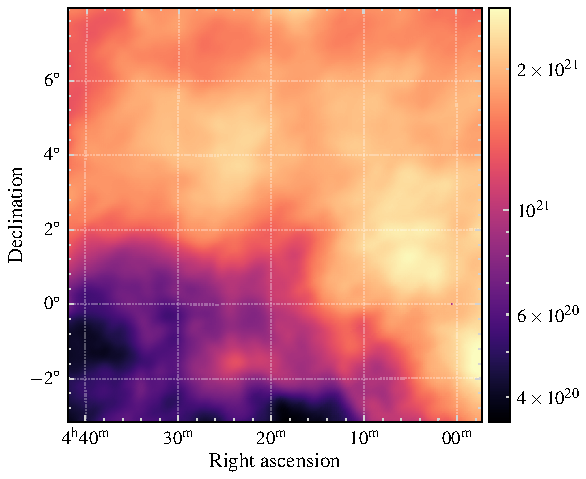
\includegraphics{appendix_a/NH_map.pdf}
    \caption[\(N_{\text{Htot}}\)-map.]{\(N_{\text{Htot}}\)-map obtained by reprojecting the HI4PI all-sky survey and querying \({\textstyle N_{\text{H}_2}}\) values from the Swift homepage. The color bar units are \(\text{cm}^{-2}\).}
    \label{fig:NH_map}
\end{figure}
%
\section{Exposure Correction}\label{sec:exposure}
The count image of any given X-ray observation is inherently dependent on a detector's effective area and the telescope's pointing motion throughout the observation. In order to obtain meaningful flux units (e.g. \(\text{cts}\cdot\text{arcsecond}^{-2}\text{s}^{-1}\)), these effects must be considered. This is accomplished by dividing the count image by the vignetted exposure map created in Section \ref{sec:exposure_map}, thereby rescaling all segments of the count image to the same relative exposure (\cite{davis2001formal}). However, an exposure map must be created separately for TM8 and TM9 for three reasons: first, TM9 uses a narrower energy band, which lowers its expected count rate; second, this narrower energy band necessitates a different absorption correction map; third, TM8 and TM9 have very distinct area response files because of their different filter configurations. Therefore, it is not possible to simply combine the two exposure maps as they must first be corrected for these effects. The procedure outlined in \citet{Reiprich2021} will be followed. 

First, the vignetted exposure map of TM8 and TM9 are divided by their respective absorption correction maps to obtain an absorption-corrected exposure map (\(\text{exmap}_\text{TM8, corr}\), \(\text{exmap}_\text{TM9, corr}\)). Second, the ratio of PIB-corrected count rates of TM8 and TM9 is used to define a correction factor 
\begin{align*}
    E_\text{corr} = \frac{\text{PIB corr. count rate(TM9)}}{\text{PIB corr. count rate(TM8)}}.
\end{align*}
The total absorption-corrected exposure map for TM0 is then given by
\begin{align*}
    \text{exmap}_\text{TM0, corr} = \text{exmap}_\text{TM8, corr} + E_\text{corr}\cdot\text{exmap}_\text{TM9, corr} 
\end{align*}
A correction factor of \(E_\text{corr} = 0.4628\) is obtained and the resulting absorption-corrected TM0 exposure map can be found in Appendix \ref{sec:appendix_a_exposure_map}. The final filtered, PIB-corrected, absorption-corrected, and exposure-corrected soft-band image is obtained by dividing the filtered and PIB-corrected soft-band TM0 image by its absorption-corrected exposure map. Henceforth, this will be referred to as the \enquote{corrected} soft-band image. An examination of the exposure map shows that the lower counts observed on the right side of each image in Figure \ref{fig:raw_photon_images} were due to a count enhancement in the left portion of each image. However, this issue has now been rectified through the absorption and exposure correction.
%
\begin{figure}[htbp]
    \centering
    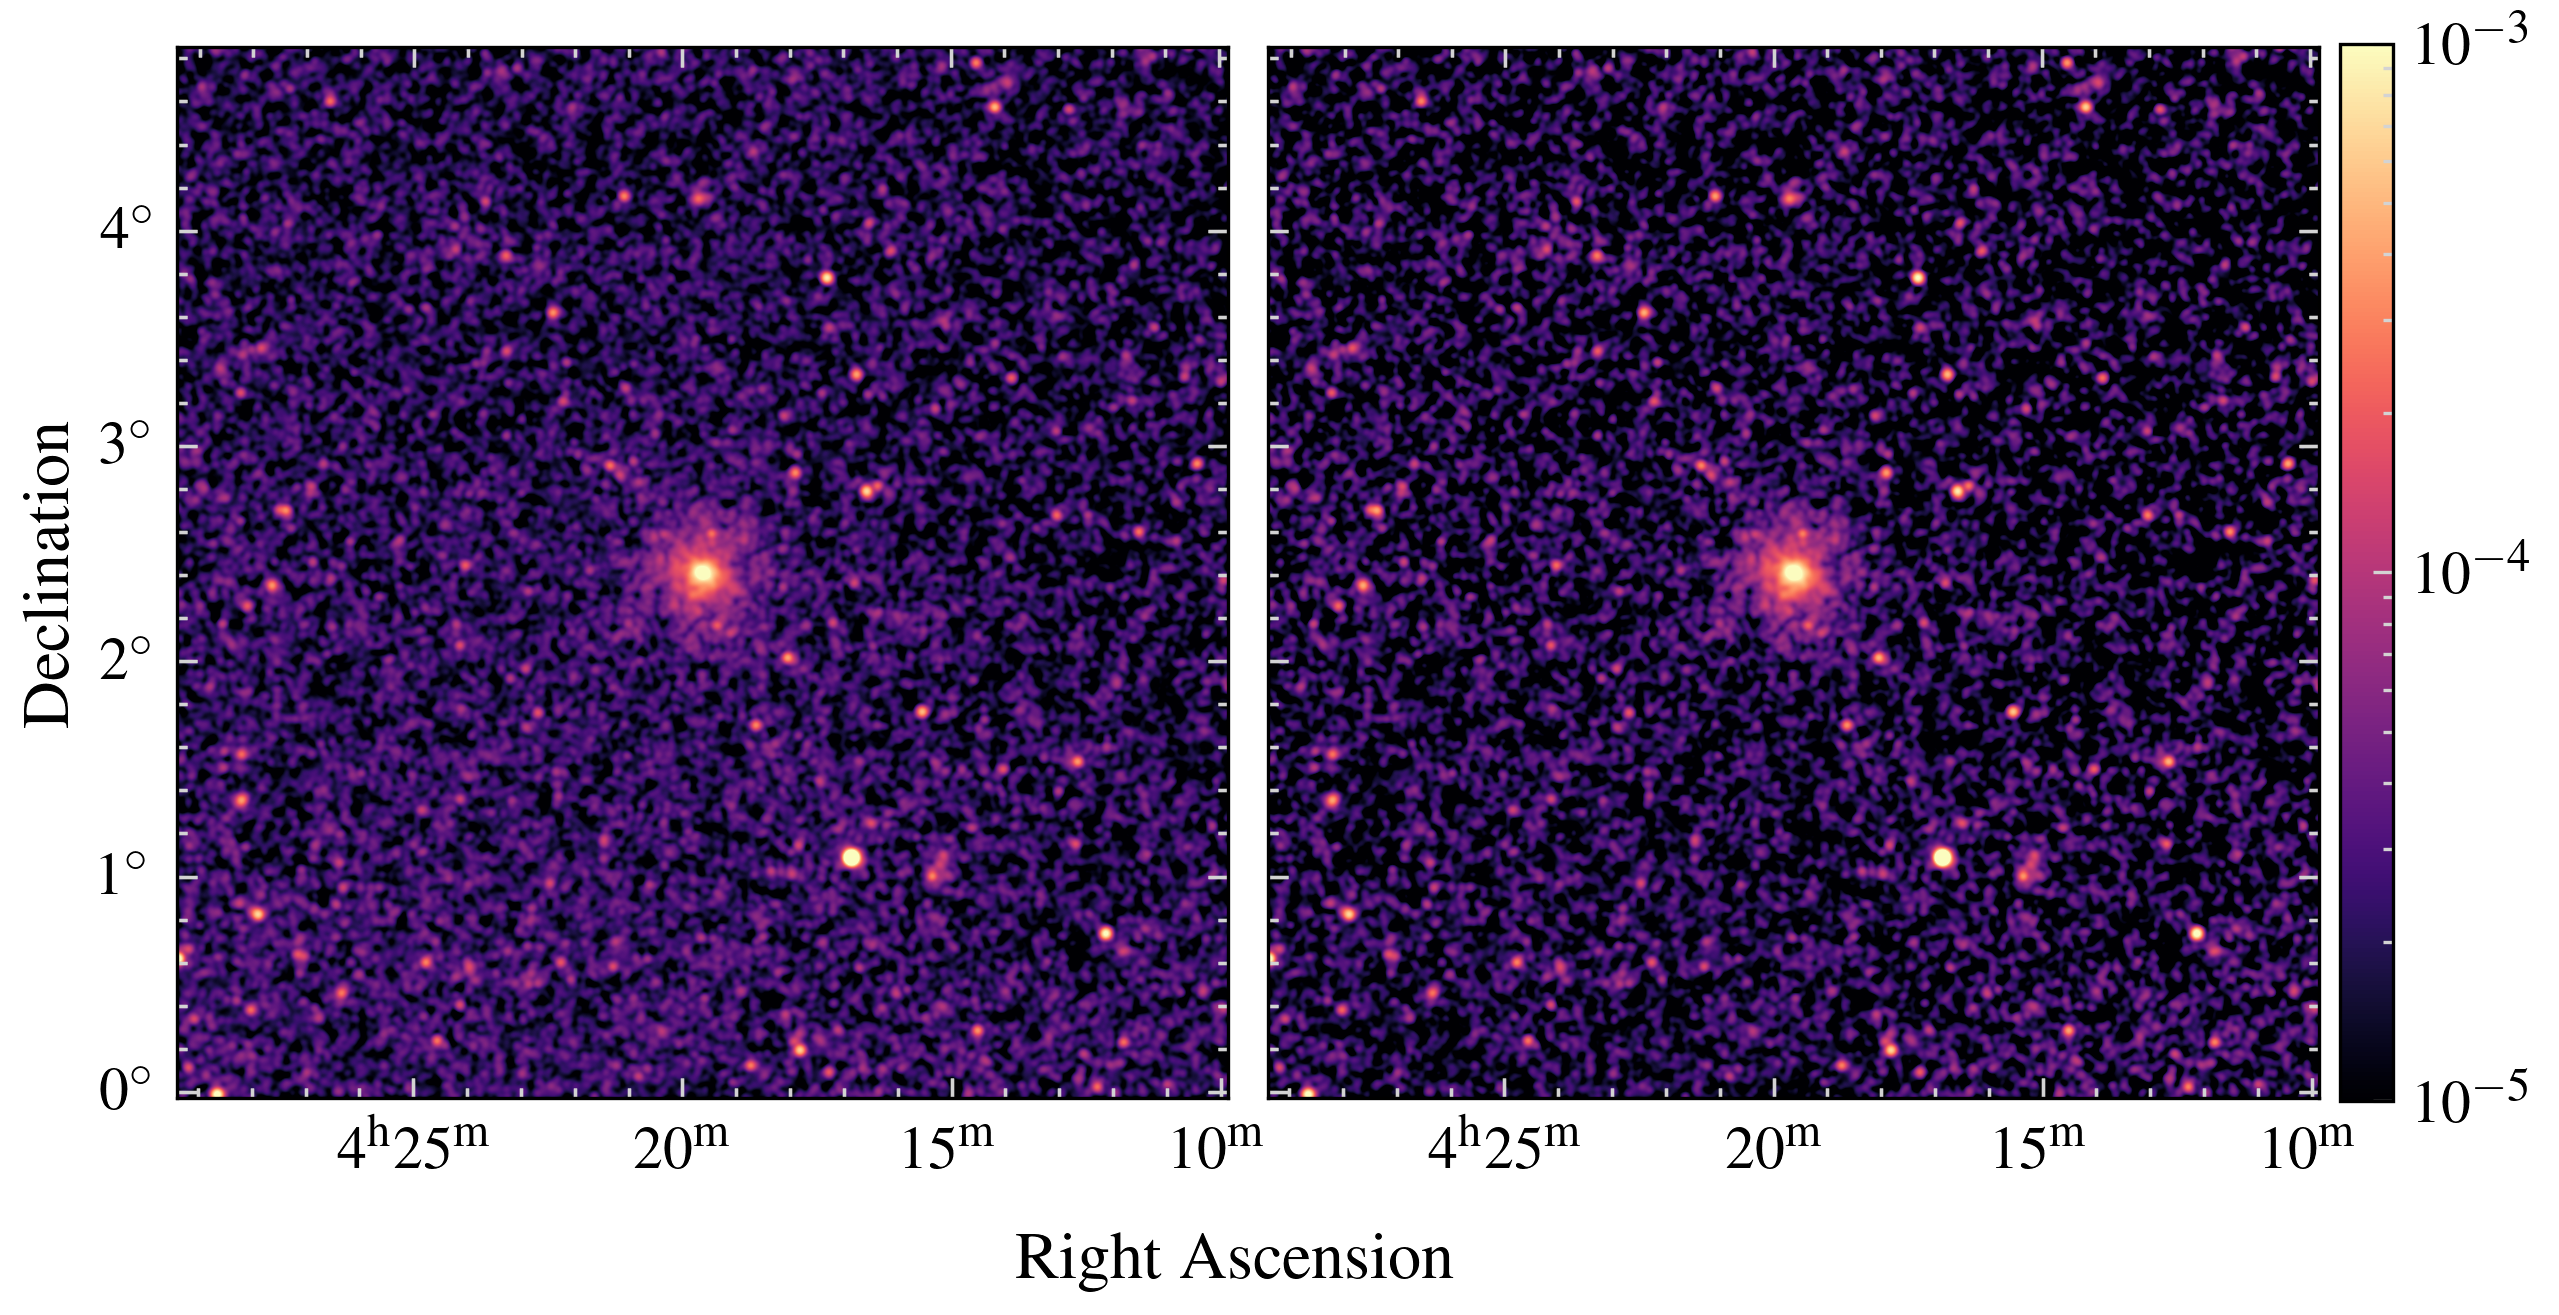
\includegraphics{data_reduction/filtered_corr_comparison.png}
    \caption[Comparison between the filtered, full energy-band count rate image and the final corrected, soft-band image.]{Comparison between the filtered, full energy-band count rate image (left) and the final corrected, soft-band count rate image (right), both smoothed using a Gaussian kernel of 12 pixels. The corrected image clearly shows improved differentiation of group emission from the background in comparison to the filtered, full band image.}
    \label{fig:comparison_filt_corr}
\end{figure}

Figure \ref{fig:comparison_filt_corr} compares the filtered, full energy-band count rate image (the filtered full band count image divided by its respective exposure map) with the corrected soft-band image, both smoothed using a Gaussian kernel of 12 pixels. It is evident that group emission can be much better distinguished from the background in the corrected soft-band image. 
%
\section{Wavelet filtering and Point Source Removal}
It is necessary to remove the emission from point-like sources (e.g. AGNs) and unrelated extended sources to avoid interfering with the group emission under study. This is achieved using the wavelet filtering pipeline as described in \citet{Pacaud2006}. The wavelet transform decomposes an image \(I(x, y)\) into coefficients \((w_1, \ldots, w_n, c_n)\)
\begin{align*}
I(x, y) = c_n(x, y) + \sum_{j=1}^{n}w_j(x, y).    
\end{align*}
Here, \(c_n(x, y)\) is the smoothed image, and \(w_j(x, y)\) essentially represents the contribution of a wavelet function at a scale \(j\) and position \((x, y)\) to the total image. By retaining only the coefficients that satisfy
\begin{align*}
|w_j(x, y)| > k\sigma_j,
\end{align*}
where \(\sigma_j\) is the standard deviation at scale \(j\) and \(k\) is a clipping factor, and then applying the inverse wavelet transform, an image is obtained that includes only significant scales, i.e. those that are not due to noise (\cite{Stark1998}). The resulting image is called a wavelet-filtered image. 

In the pipeline being used, the absorption-corrected exposure map, \(\text{exmap}_\text{TM0, corr}\), and the filtered photon image are used to account for the previous data reduction and to statistically treat the Poisson noise. After wavelet filtering, a source catalog is obtained by \texttt{SExtractor} (\cite{Bertin1996}). This is made possible by the significant noise reduction and smoothed background achieved by the wavelet filtering. The extended X-ray emission near NGC1550 is manually removed from the catalog, and a cheese mask is created from the catalog and applied to \(\text{exmap}_\text{TM0, corr}\). Emission around unrelated, but projectionally close, clusters and groups is also manually added to the cheese mask. Repeating the wavelet filtering with the cheese-masked map reduces ringing artifacts that typically occur near bright sources with steep flux gradients, and allows the detection of the previously missed sources. Figure \ref{fig:comparison_wvl_filtered} compares the wavelet filtering before and after applying of the cheese mask to the exposure map. Furthermore, the complete data reduction workflow described in this chapter is briefly summarized in Figure \ref{fig:good_soup}
%
\begin{figure}[htbp]
    \centering
    \begin{subfigure}[b]{0.48\textwidth}
        \centering
        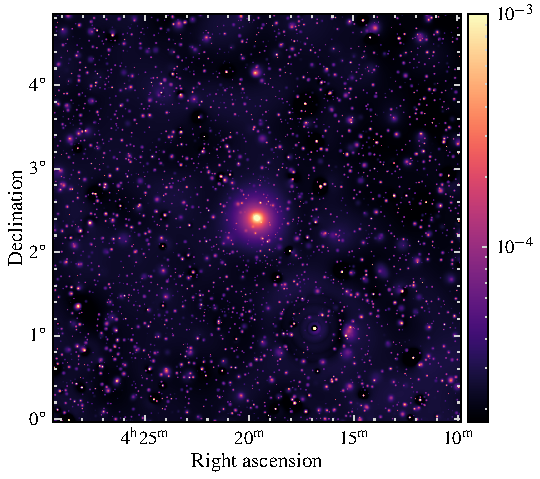
\includegraphics[width=\textwidth]{data_reduction/wlt_filtered.pdf}
        \caption{Before applying the cheese-mask}
        \label{fig:wlt_filtered}
    \end{subfigure}
    \hfill
    \begin{subfigure}[b]{0.48\textwidth}
        \centering
        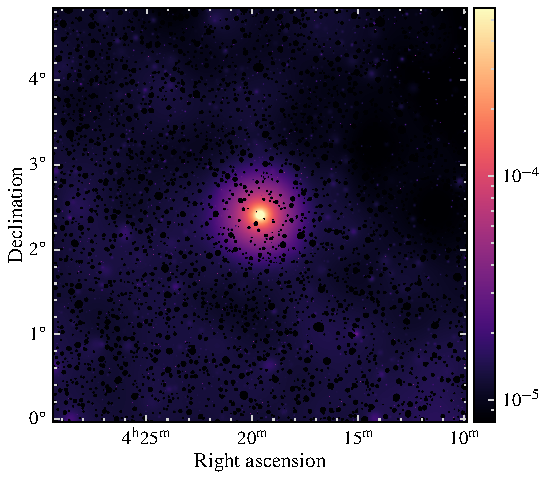
\includegraphics[width=\textwidth]{data_reduction/wlt_filtered_cheese.pdf}
        \caption{After applying the cheese-mask}
        \label{fig:wvl_filtered_cheesed}
    \end{subfigure}
    \caption[Corrected wavelet filtered image before and after applying the cheesemask.]{Corrected wavelet filtered image before (a) and after (b) applying the cheesemask. The left image is normalized such that the ringing artifacts are more prominent. The cheese-masked image has significantly reduced ringing artifact and group emission is well visible.}
    \label{fig:comparison_wvl_filtered}
\end{figure}
%
\begin{figure}[htbp]
    \centering
    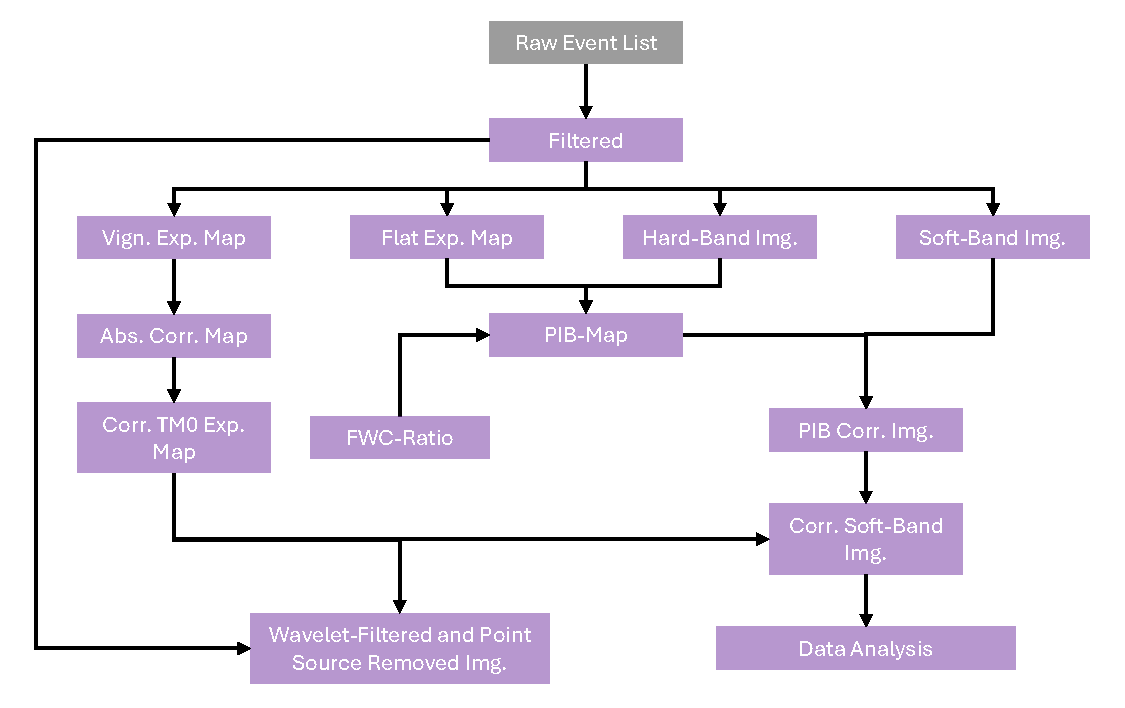
\includegraphics[width=\textwidth]{data_reduction/eROSITA-workflow.pdf}
    \caption[Workflow diagram of the data reduction procedures.]{Workflow diagram summarizing the data reduction procedures described in this chapter.}
    \label{fig:good_soup}
\end{figure}






%------------------------------------------------------------------------------

% !TEX root = mythesis.tex

%==============================================================================
\chapter{Data Analysis}
\label{sec:data_analysis}
%==============================================================================
\section{Image Visual Inspection}
\section{Surface Brightness Analysis}
\subsection{Full Azimuthal Surface Brightness Analysis}
\begin{figure}[htbp]
    \centering
    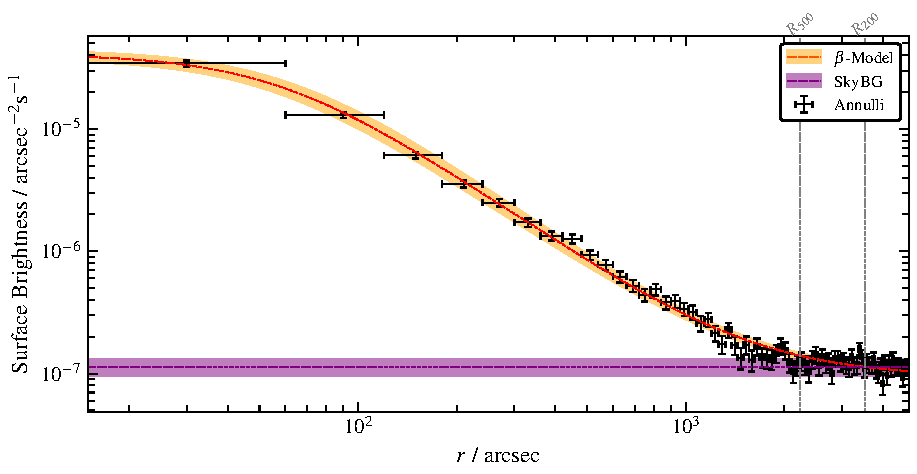
\includegraphics{data_analysis/beta_model_tot_surf_bri_anulli1_1arcmin.pdf}
    \caption{A nice plot.}
\end{figure}
To accurately quantify potential asymmetries in the X-ray emission of NGC 1550, surface brightness analysis is performed. First, the emission center is estimated by constructing a \(2'\) aperture around the apparent center, as given in Section X. This aperture size is chosen to capture a statistically significant number of photons while minimizing bias from potential asymmetries outside the group center. The flux-weighted average of the image coordinates within this aperture yields a right ascension of \SI{64.909}{\degree} and a declination of \SI{2.414}{\degree}. Concentric Anulli with \(1'\) width are constructed from the calculated flux-weighted surface brightness of the group up to \(80'\). The counts \(C\) within each annulus are determined using the \texttt{funcnts} task from the \texttt{funtools} software, with a Poisson error of \(\sqrt{C}\). The surface brightness \(S\) for each annulus is calculated by
\begin{align*}
    S = \frac{C_\text{image} - C_\text{PIB}}{C_\text{expmap}\cdot A},
\end{align*}
where \(C\) denotes the counts in the photon image, total PIB map, and exposure map, respectively. Errors are calculated using Gaussian error propagation. Furthermore,background estimation is performed using \(10\) circular regions with a \(48'\) radius, each centered \(160'\) from the calculated center of NGC 1550. The average background surface brightness is evaluated for all circles combined and separately for the northern (Circles 1-5) and southern regions (Circles 6-10) to account for possible background gradients. 


%------------------------------------------------------------------------------

% !TEX root = mythesis.tex

%==============================================================================
\chapter{Conclusion}
\label{sec:conclusion}
%============================================================
The aim of this thesis was the characterization of the X-ray morphology of the galaxy group NGC1550 through detailed surface brightness analysis. After correcting and reducing the raw photon data obtained from eRASS:1 in Chapter \ref{sec:data_reduction}, Chapter \ref{sec:data_analysis} began with qualitative inspection of the corrected data. A contour plot of the corrected, cheese-masked wavelet filtered image in the soft-band with an overlaid galaxy distribution was shown (Figure \ref{fig:contour_wvl_filtered}). From this figure, it was visually established that the galaxy group NGC1550 appears relaxed and spherically symmetrical. Furthermore, using a contour plot of the corrected soft-band image (Figure \ref{fig:contour_fully_corrected}), some indications of asymmetry were visually identified within \(810''\). Emission was found to drop off to background levels at \(R_{500}\) and a complex background was noted, which can be attributed to the Orion-Eridanus superbubble. No obvious correlation between the X-ray contours and the galaxy distribution could be ascertained.

To more accurately characterize the morphology of NGC1550 in the X-ray, surface brightness analysis was performed. A beta model was fitted to characterize the full azimuthal profile, as shown in Figure \ref{fig:tot_azimuthal_beta_model}. The model fitting yielded a \(\beta\)-value of \(0.478 \pm 0.008\) and a core radius of \(r_c = (60 \pm 5)'' \approx (15\pm2)\,\text{kpc}\) with a reduced chi-squared value of \(0.96\), indicating a good fit. This result was consistent with the findings of previous studies, showing that the eROSITA view of NGC1550 aligns with previous findings. The full azimuthal surface brightness profile showed no significant deviations from spherical symmetry. Moreover, the sectoral surface brightness analysis across the north, south, east, and west sectors, as well as the combined north-south and east-west sectors, also revealed no significant deviations from azimuthal symmetry beyond \(390''\).

The residual image indicated that the beta model does not described emission within \(R_{500}\) accurately, underestimating the core emission, as is common, and no features were detected. Attempts to use a two beta model were unsuccessful, likely due to the large width of the annuli and the small inner core component, which, from previous studies (\cite{Kawaharada_2009}), is of order of eROSITA's angular resolution. 

Within \(390''\), the qualitatively observed east-west elongation could not be quantitatively confirmed by the surface brightness analysis. Although the sectoral surface brightness profiles did not differ significantly from the azimuthal profile, their fit parameters often varied significantly and the individual beta fits of each sector were of slightly lower quality (\(\chi^2 \lesssim 0.8\)). It was speculated that these issues were caused by the fairly wide \(1'\) anulli and due to a poor choice of the SB-center, resulting in a significant discrepancy between the north and south emission for the first data point at \(\sim 1'\). The surface brightness analysis also highlighted a slight discrepancy between the observationally estimated backgrounds and the fitted background levels, suggesting that background estimation could have been performed with greater care.   
\section{Outlook}
After analyzing the results of this thesis, some suggestions for improvement can be made. The SB-center could have been determined more precisely, either manually or, better, by a two-dimensional beta fit of the full azimuthal profile, allowing it to be freely fitted. A comparison using the brightest pixel as the SB-center is ongoing work and will be presented at a later date. Better background estimation using different background regions could also have been attempted, and visualization of the background gradient by plotting the background emission of each circular region may also be interesting. 

Furthermore, because only eRASS:1 data was utilized, several features observed qualitatively, such as a slight emission dip in the western sector between \(\sim 390''\) and \(\sim 810''\), could not be verified quantitatively. With additional data, such as from eRASS:4, these features could be more accurately interpreted and their significance better assessed. The increased data would also allow for finer annuli in the surface brightness analysis due to the higher count rates in each annulus bin, thus facilitating feature identifications. Although no evidence was found in this work, additional data with better statistics may reveal other features in the soft-band, such as filaments in the outskirts \citep{Cen_1999}. Additionally, enabled by eROSITA's wide field of view and great sensitivity in the soft-band, future work could study superbubbles such as Orion-Eridanus, as has been done in previous studies with ROSAT data \citep{Krause_2014}. 

%------------------------------------------------------------------------------
\appendix
\part*{Appendix}
% Add your appendices here - don't forget to also add them to \includeonly above
\chapter{Appendix}
\section{PIB Map}\label{sec:appendix_a_pib_map}
\begin{figure}[htbp]
    \centering
    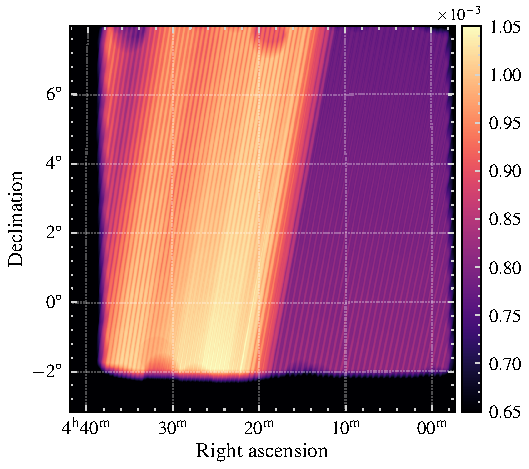
\includegraphics{data_reduction/PIB_MAP.pdf}
    \caption{PIB map created by co-adding individual background maps for each telescope module (TM).}
    \label{fig:pib_map}
\end{figure}
%------------------------------------------------------------------------------
% Use biblatex for the bibliography.
% Add bibliography to Table of Contents.
% Use this command  (and remove refsection environments)
% to print all references at the end of the thesis.
\printbibliography[heading=bibintoc]


%------------------------------------------------------------------------------
% Declare lists of figures and tables and acknowledgements as backmatter
% Chapter/section numbers are turned off
\backmatter

\listoffigures
\listoftables

%------------------------------------------------------------------------------
% Print the glossary and list of acronyms
% \printglossaries

%------------------------------------------------------------------------------
% You could instead add your acknowledgements here - don't forget to
% also add them to \includeonly above
% %------------------------------------------------------------------------------
\chapter*{Acknowledgements}
\label{sec:ack}
%------------------------------------------------------------------------------

I would like to thank ...

You should probably use \texttt{\textbackslash chapter*} for
acknowledgements at the beginning of a thesis and
\texttt{\textbackslash chapter} for the end.

%%% Local Variables: 
%%% mode: latex
%%% TeX-master: "../mythesis"
%%% End: 


\end{document}
